\documentclass[12pt]{article}

% #################### PREAMBLE ##########################

% Global margins for the document:
\usepackage[margin=0.6cm]{geometry}

% Define spacing between paragraphs in the document:
\setlength{\parindent}{0.5cm} % default indentation before the first line of a paragraph.
\setlength{\topskip}{0.2cm} % indentation at the begging of the first paragraph of every page:
\setlength{\parskip}{0.3cm} % indentation after every paragraph

% Font configurations:
\usepackage{fontspec}
\setmainfont{FreeSerif}

% For justify and some other alignment extensions:
\usepackage{ragged2e}

% Math related packages:
\usepackage{amsmath, amssymb, amsthm}

% Embedding *.jpg abd *.png images
\usepackage{graphicx}
\graphicspath{{data/}{../data/}} % define the path to the images

% Provides an underline command which will break over line ends:
\usepackage{ulem}

% Better lines for tables:
\usepackage{hhline}

% To use arrays:
\usepackage{array}

% Custom commands for table alignment when dealing with a lot of text (needs array and ragged2e):
\newcolumntype{L}[1]{>{\raggedright\let\newline\\\arraybackslash\hspace{0pt}}m{#1}}
\newcolumntype{C}[1]{>{\centering\let\newline\\\arraybackslash\hspace{0pt}}m{#1}}
\newcolumntype{R}[1]{>{\raggedleft\let\newline\\\arraybackslash\hspace{0pt}}m{#1}}

% Hyper links to places inside the document:
\usepackage{hyperref}
\hypersetup{
    colorlinks=true,
    % These take rgb values as a fraction of n/255.
    % That is really not how RGB works!
    linkcolor=[rgb]{0.1, 0.2, 1},
    filecolor=[rgb]{0.1, 0.2, 1},
    urlcolor=[rgb]{0.1, 0.2, 1},
    citecolor=[rgb]{0.1, 0.2, 1},
    unicode=true,
}
\urlstyle{same}

% For pretty quotes:
\usepackage{epigraph}
\setlength\epigraphwidth{1\textwidth}
\setlength\epigraphrule{0pt}

% Bibliography:
\usepackage{csquotes}
\usepackage[backend=biber]{biblatex}
\addbibresource{init.bib}

% For inserting loremipsum random text:
\usepackage[pangram]{blindtext}

% Allows adding sub tex files to the main tex file:
\usepackage{subfiles} % Best loaded last in the preamble

% #################### DOCUMENT BEGIN ####################

\begin{document}

\begin{center}
    {\Huge Big Centered Text}
\end{center}

1. Tiny noindent text: \\
{\tiny\noindent\Blindtext[1][1]}

2. Scriptsize text with added additional 4cm indentation, which is then removed -4cm:

\addtolength{\parindent}{4cm}
{\scriptsize\Blindtext[1][1]}
\addtolength{\parindent}{-4cm}

3. Footnotesize flush right text:
\begin{flushright}
{\footnotesize\Blindtext[1][1]}
\end{flushright}

4. Normalsize flus left text:
\begin{flushleft}
{\normalsize Something in this document. This paragraph contains no information and its purposes is to provide an example on how to insert white spaces and lines breaks. Right here -> \textbackslash\textbackslash \\
When a line break is inserted, the text is not indented, there are a couple of commands for line breaks. \textbackslash newline \newline
This paragraph contains full line break. \textbackslash hfill and \textbackslash break \hfill \break For combining two commands}
\end{flushleft}

5. large centered text:
\begin{center}
{\large Nisi qui culpa pariatur velit deserunt nulla nulla dolor cillum est do nulla ut. Nisi qui culpa pariatur velit deserunt nulla nulla dolor cillum est do nulla ut.}
\end{center}

6. Large text after 2 newlines (baselineskip) : \\[2\baselineskip]

{\Large The environments center, flushleft, flushright, justify should only be used with text paragraphs. They can NOT format other LaTeX objects!}

7. Graphics with set width 0.3 of linewidth:
\begin{center}
    
\includegraphics[width=0.3\linewidth]{sample.png}
\end{center}

\newpage

\tableofcontents
\listoffigures
\listoftables
\setcounter{section}{8}

\newpage

\section{Images and figures}

\subsection{LaTeX includegraphics wrapped in a figure}
\begin{figure}[ht!]
    \centering
    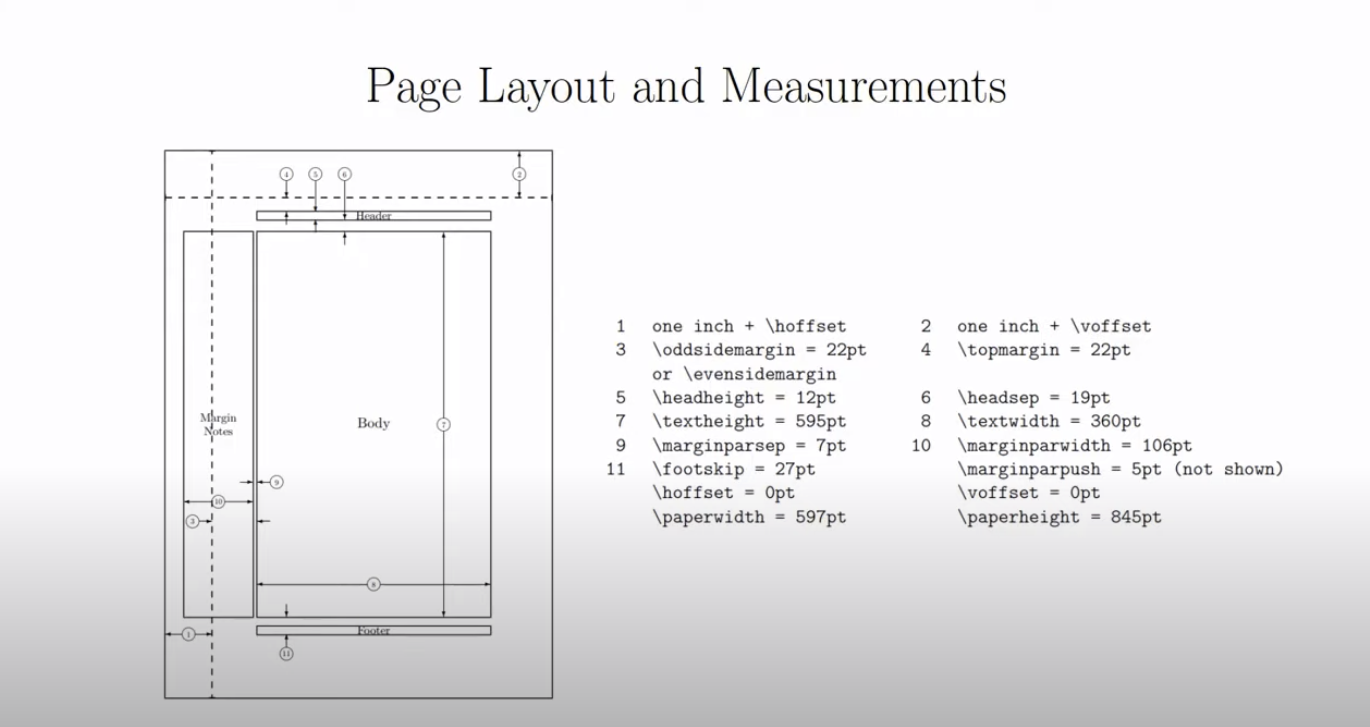
\includegraphics[width=\linewidth]{page_layout.png}
    \caption{LaTeX Page layout and Measurements (width=linewidth)}
    \label{hr_3}
\end{figure}

\section{Section with subsections}

\subsection{LARGE text}
{\LARGE \indent Nisi qui culpa pariatur velit deserunt nulla nulla dolor cillum est do nulla ut. Nisi qui culpa pariatur velit deserunt nulla nulla dolor cillum est do nulla ut.}

\subsection{huge text with bold, italic and standard underline}
{\huge \indent Nisi qui \textbf{culpa} \textit{pariatur} \underline{velit deserunt} nulla nulla dolor cillum est do nulla ut.} \\

\subsection{Huge text with combined bold, italic and standard underline}
{\Huge \indent Nisi qui culpa pariatur velit deserunt \underline{\textbf{\textit{nulla dolor cillum est}}} do nulla ut.} \\

\subsection{This is what happens when you underline long text}
\underline{\textbf{Unerlining a long string of text is kinda hard in latex with the default underline so we can use ulem}. Nisi qui culpa pariatur velit deserunt nulla nulla dolor cillum est do nulla ut. Nisi qui culpa pariatur velit deserunt nulla nulla dolor cillum est do nulla ut.} \\

\subsection{We can fix the above problem with the package ulem using uline}
\uline{\textbf{Same with ulem}. Nisi qui culpa pariatur velit deserunt nulla nulla dolor cillum est do nulla ut. Nisi qui culpa pariatur velit deserunt nulla nulla dolor cillum est do nulla ut.}

{\large \noindent ulem also has \uuline{some other} cool \uwave{underlines}.}

\subfile{sections/citations.tex}

\section{Basic Math Equations}

\subsection{Displaystyle math equation}

\begin{equation} % equivalent to $$ .. $$
    \sum_{n=1}^\infty \frac{1}{n^2} = \frac{\pi^2}{6}
\end{equation}

\subsection{Inline math with display style mode}

Ex qui anim eu consequat est excepteur ea est. Exercitation officia pariatur pariatur nostrud. Cillum cillum proident minim officia ex. Aliquip ut officia sit voluptate quis dolor sint proident tempor aliquip qui enim. $ \displaystyle \sum_{n=1}^\infty \frac{1}{n^2} = \frac{\pi^2}{6} $ Elit veniam minim commodo proident do aliqua Lorem sunt ex dolore. Irure adipisicing enim eu velit eiusmod reprehenderit. Sit exercitation minim sunt et.

\subsection{Inline math with text style mode}

Ex qui anim eu consequat est excepteur ea est. Exercitation officia pariatur pariatur nostrud. Cillum cillum proident minim officia ex. Aliquip ut officia sit voluptate quis dolor sint proident tempor aliquip qui enim. $ \textstyle \sum_{n=1}^\infty \frac{1}{n^2} = \frac{\pi^2}{6} $ Elit veniam minim commodo proident do aliqua Lorem sunt ex dolore. Irure adipisicing enim eu velit eiusmod reprehenderit. Sit exercitation minim sunt et.

\subsection{Brakets sizes}

These are a bit unreadable:
\begin{equation*}
    ( \sum_{n=0}^N ( \frac{1}{a + b} )^2 )^2
\end{equation*}

\noindent We can use left and right braket:
\begin{equation*}
    \left( \sum_{n=0}^N \left( \frac{1}{a + b} \right)^2 \right)^2
\end{equation*}

\section{Tables and Arrays}

\subsection{Simple Tables}

\begin{tabular}{lcr}
    left justified & centered & right justified \\
    l & c & r
\end{tabular}

\noindent Table with boarders \\

\noindent
\begin{tabular}{ | l |c r| }
    \hline
    left justified & centered & right justified \\
    \hline
    l & c & r \\
    \hline
\end{tabular}

\noindent Note that begin center is quite limited for tables, but can work for a quick and simple solution sometimes: \\
\begin{center}
    \begin{tabular}{ | l |c r| }
        \hhline{ | - | - | - | }
        left justified & centered & right justified \\
        \hhline{ | - | ~ - | }
        l & c & r \\
        \hhline{ | - | ~ - | }
    \end{tabular}
\end{center}

\subsection{Long text in column and other table packages}

This problem: \\
\begin{tabular}{ | l | c | r | }
    \hline
    long text in table long text in table long text in table long text in table long text in table long text in table long text in table long text in table long text in table &
    long text in table long text in table long text in table long text in table long text in table long text in table long text in table long text in table long text in table &
    long text in table long text in table long text in table long text in table long text in table long text in table long text in table long text in table long text in table
    \\
    \hline
\end{tabular}

\noindent Can be fixed like this, with 3 custom commands defined in the preamble:

\begin{tabular}{ | L{5cm} | C{4cm} | R{3cm} | L{4cm} | }
    \hline
    For more advanced tables we can use the \textbf{\textbackslash usepackage\{booktabs\}} - Provides extra commands to make tables more attractive &
    For more advanced tables we can use \textbf{\textbackslash usepackage\{tabularx\}}, which provides another way to control the width of the columns &
    For more advanced tables we can use \textbf{\textbackslash usepackage\{colortbl\}} to add color to tables, including line colors and cell background colors &
    For more advanced tables we can use \textbf{\textbackslash usepackage\{longtable\}} for large tables that span across multiple pages
    \\
    \hline
\end{tabular}

% BIB:
\newpage
\printbibliography

\end{document}